\documentclass[12p, Times New Roman]{beamer}
\usepackage[utf8]{inputenc} 
\usepackage[croatian]{babel}
\usepackage{graphicx}
\usetheme{Ilmenau}

\title{Github vs Bitbucket}
\author{Luka Otović, Ivo Santini, Mauro Copetti}
\date{12.siječnja 2018.}
\institute{Tehnički fakultet Rijeka}

\logo{
\includegraphics[scale=0.3]{logo.png}}

\begin{document}
	
	\frame{\titlepage}			% frame 0
	
	\begin{frame}     			% frame 1                                    
		\frametitle{GitHub}

		\begin{itemize}
			\item Tom Preston-Werner, Chris Wanstrath i PJ Hyett su ga objavili
		u travnju 2008. godine
			\item web-baziran je Git servis za kontrolu verzija
			\item koriste ga programeri u različite svrhe
		\end{itemize}

	\begin{figure}[h!]
		\begin{center}
			
\includegraphics[scale=0.10]{macka.png}
			\caption{Logo GitHub-a}
		\end{center}
	\end{figure}

	\end{frame}       

	\begin{frame}				% frame 2
		\frametitle{GitHub}
		\begin{itemize}
			\item najveći je domaćin izvornog koda u svijetu premašujući
	20 miljuna korisnika i 57 miljuna repozitorija
			\item vrijedi preko 2 milijarde USD

		\end{itemize}

		\begin{figure}[h!]
			\begin{center}
				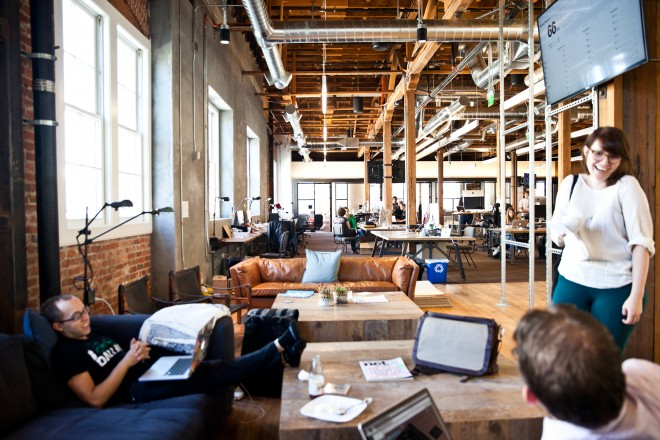
\includegraphics[scale=0.25]{headqgit.png}
				\caption{Sjedište GitHub-a}
			\end{center}
		\end{figure}


	\end{frame}



	\begin{frame}      			% frame 3        
		\frametitle{Bitbucket}

		\begin{itemize}
			\item osnovao ga je Jesper Nohr 2008. godine, a kasnije ga kupuje Atlassian
			\item web-baziran je Git i Mercurial servis za kontrolu verzija
			\item koristi se poput GitHub-a

		\end{itemize}

		\begin{figure}[h!]
			\begin{center}
				
\includegraphics[scale=0.04]{Bitbucket.png}
				\caption{Logo Bitbucket-a}
			\end{center}
		\end{figure}

	\end{frame}                



	\begin{frame}				% frame 4
		\frametitle{Bitbucket}
		\begin{itemize}
			\item ima 5 milijuna korisnika
			\item vrijedi 160 milijuna USD

		\end{itemize}

		\begin{figure}[h!]
			\begin{center}
				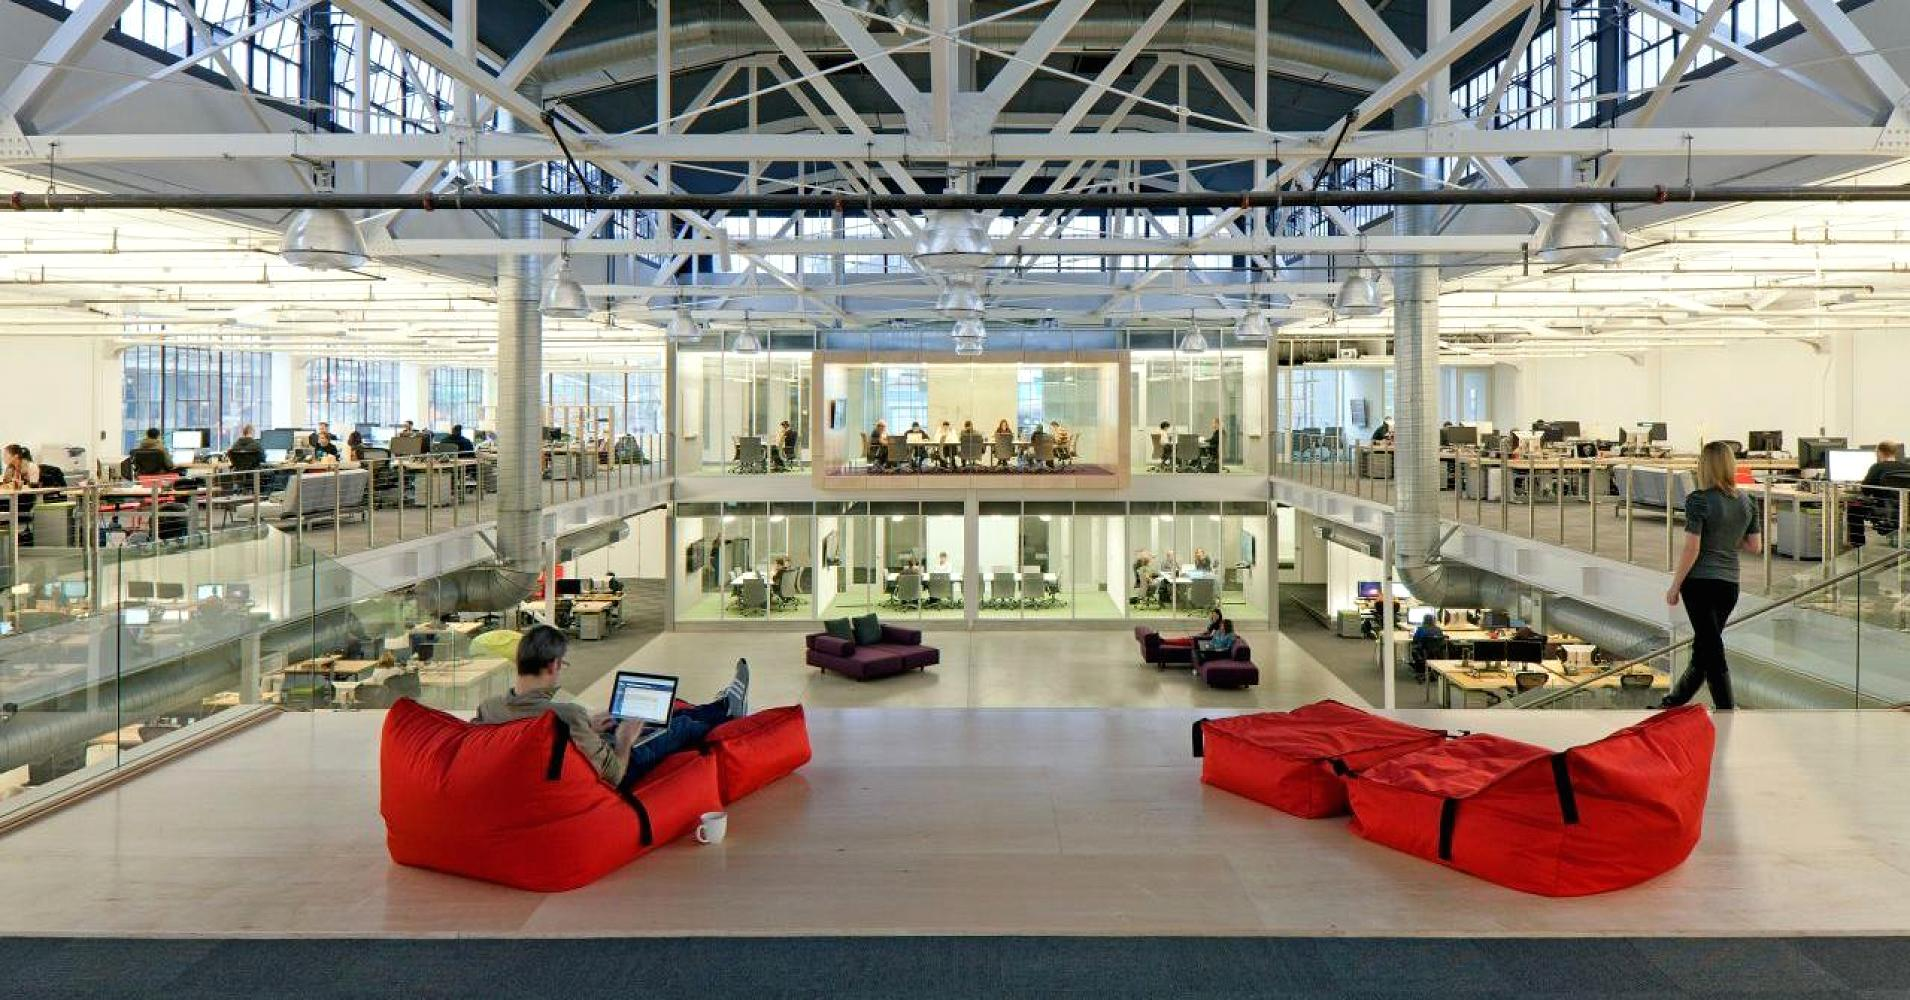
\includegraphics[scale=0.135]{headqbit.png}
				\caption{Sjedište Atlassian-a}
			\end{center}
		\end{figure}


	\end{frame}




	\begin{frame}    		    % frame 5
		\frametitle{GitHub vs Bitbucket}

		 \begin{figure}[h!]
			\begin{center}
				
\includegraphics[scale=0.34]{GVB.png}
			\end{center}
		\end{figure}
 


	\end{frame}                             


	\begin{frame} 			   % frame 6	
		\frametitle{Dizajn (GitHub)}
		
		\begin{figure}
			\begin{center}
				
\includegraphics[scale=0.1]{macka.png}
			\end{center}
		\end{figure}

	\end{frame}                              




	\begin{frame}				% frame 7
		\frametitle{Dizajn (Bitbucket)} 	
		\begin{figure}
			\begin{center}
				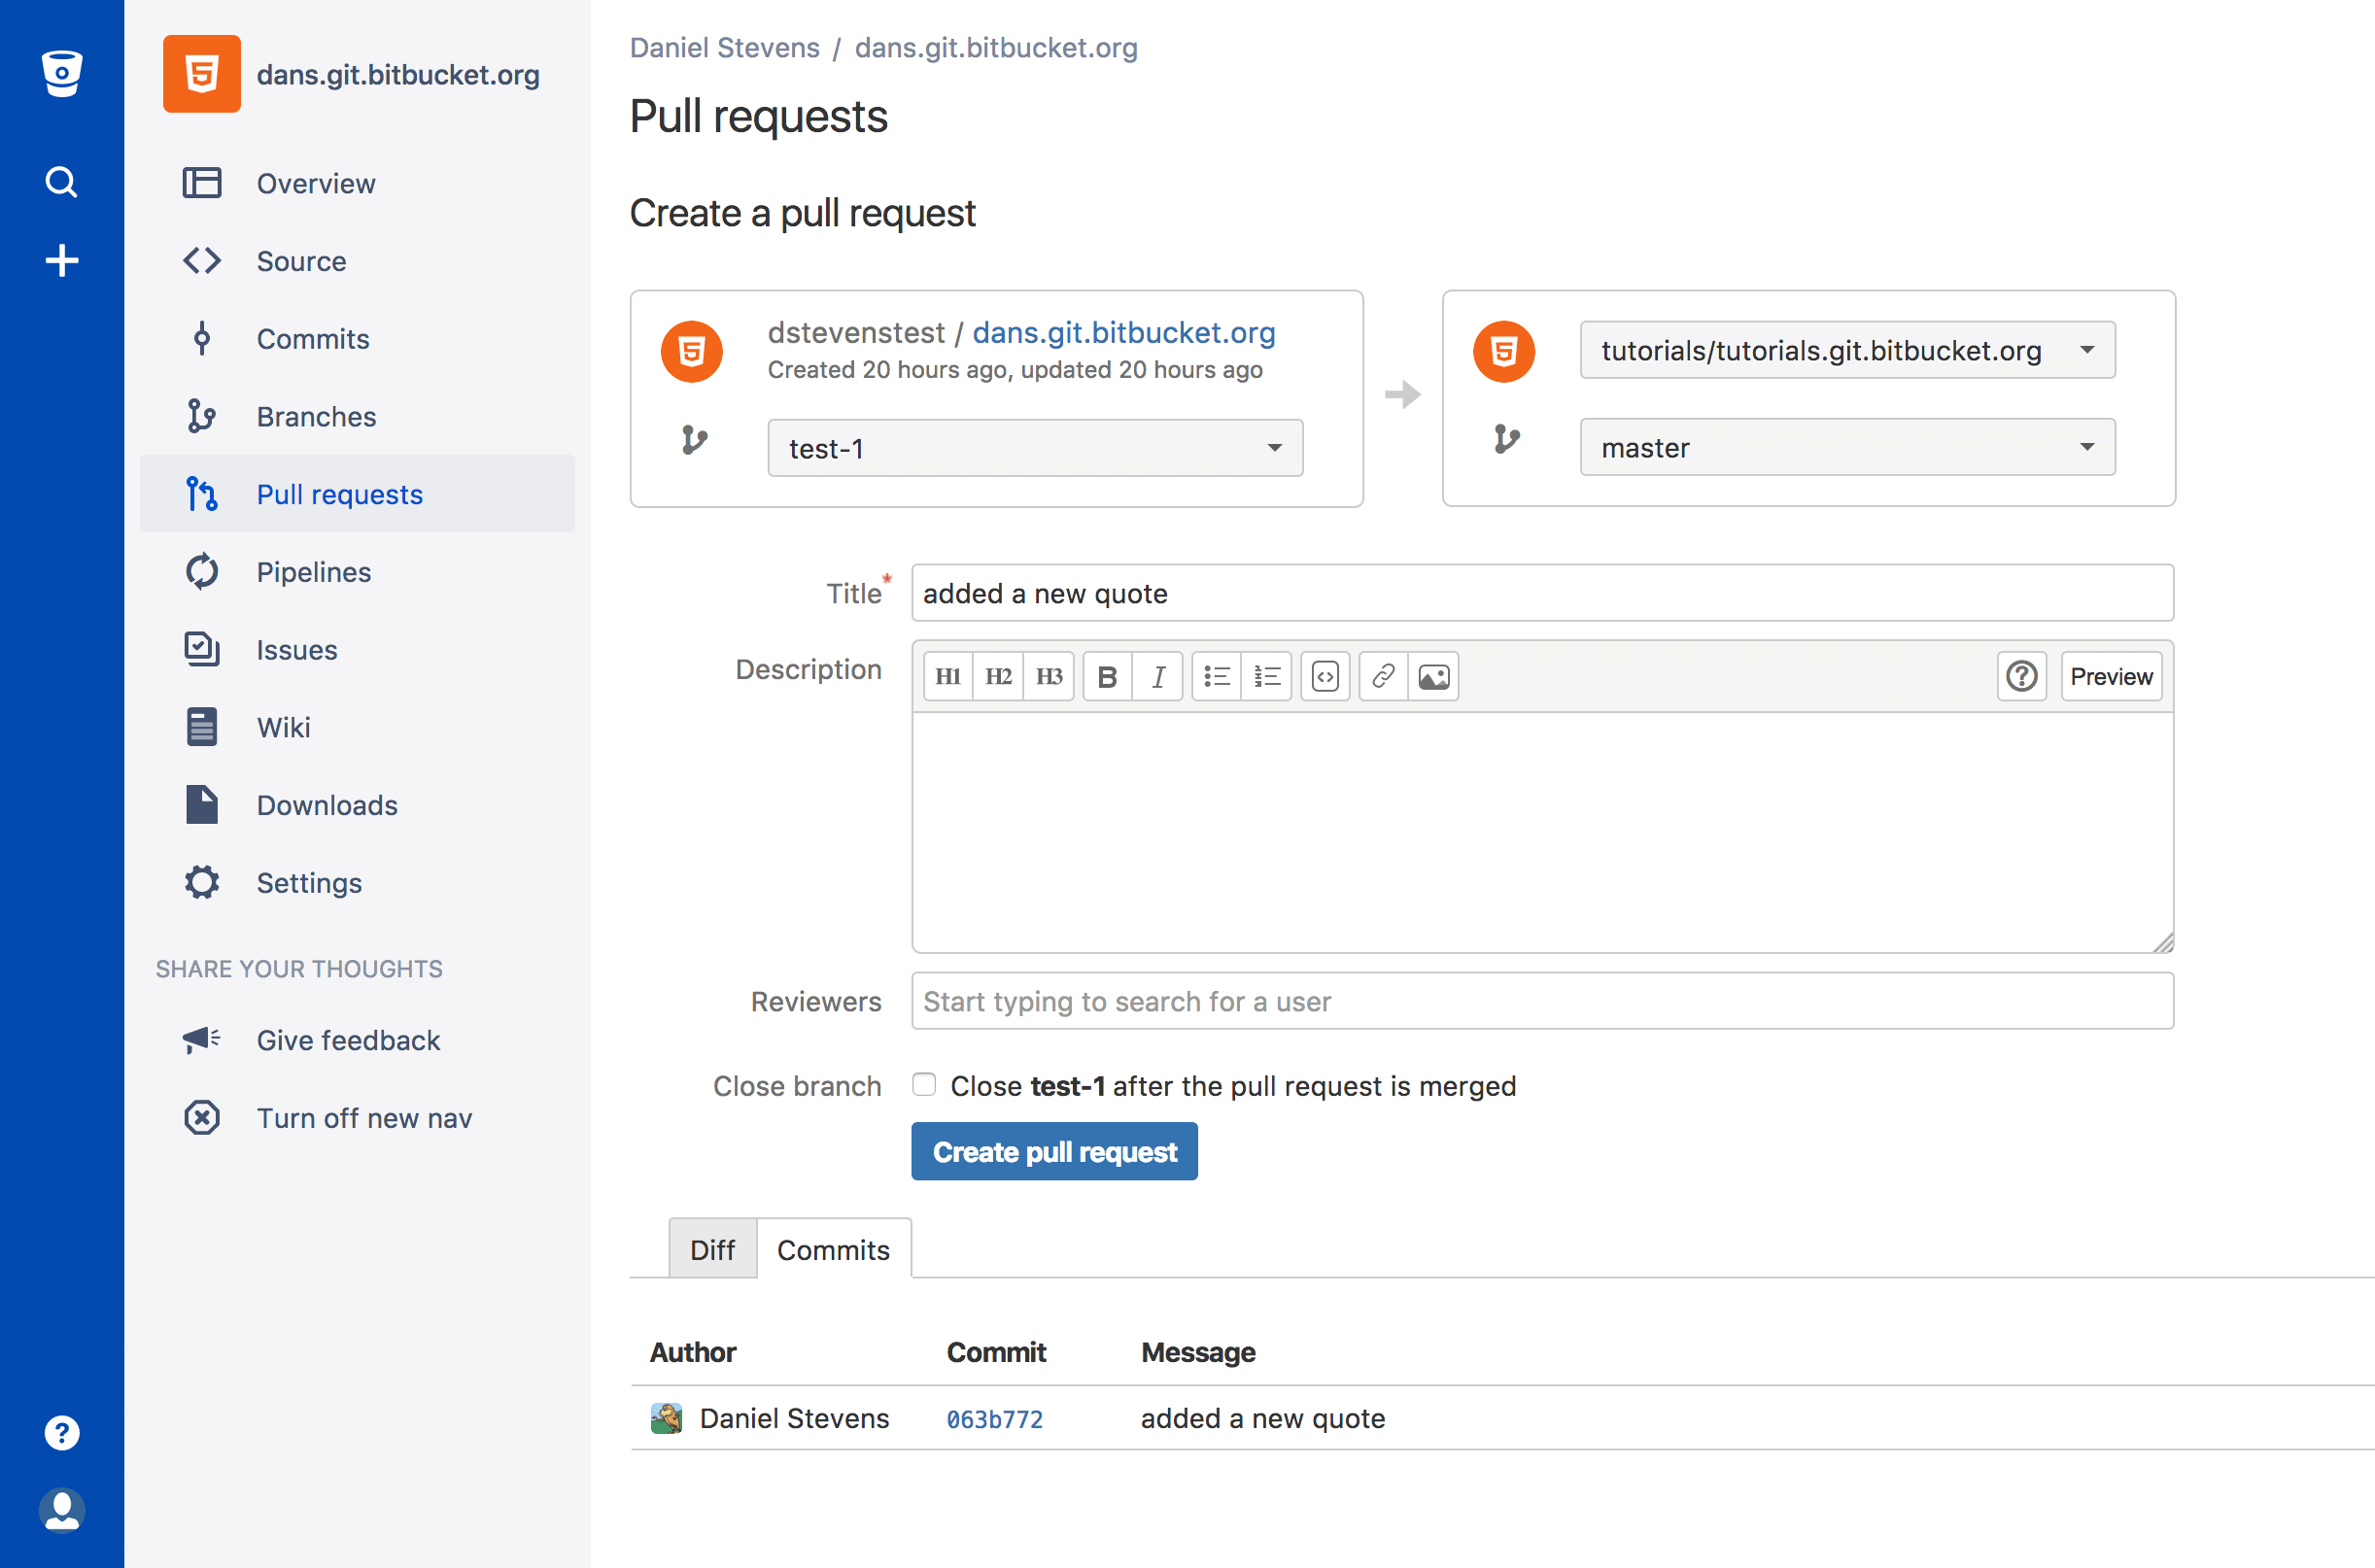
\includegraphics[scale=0.12]{Shot2.png}
			\end{center}
		\end{figure}

	\end{frame}

	\begin{frame}				% frame 8
		\frametitle{Cijene usluga (GitHub)}

		\begin{itemize}
			\item s besplatnom verzijom dobivamo javni repozitorij s beskonačno članova
			\item ako dodatno platimo dobivamo razne mogućnosti

		\end{itemize}

		\begin{figure}
			\begin{center}
				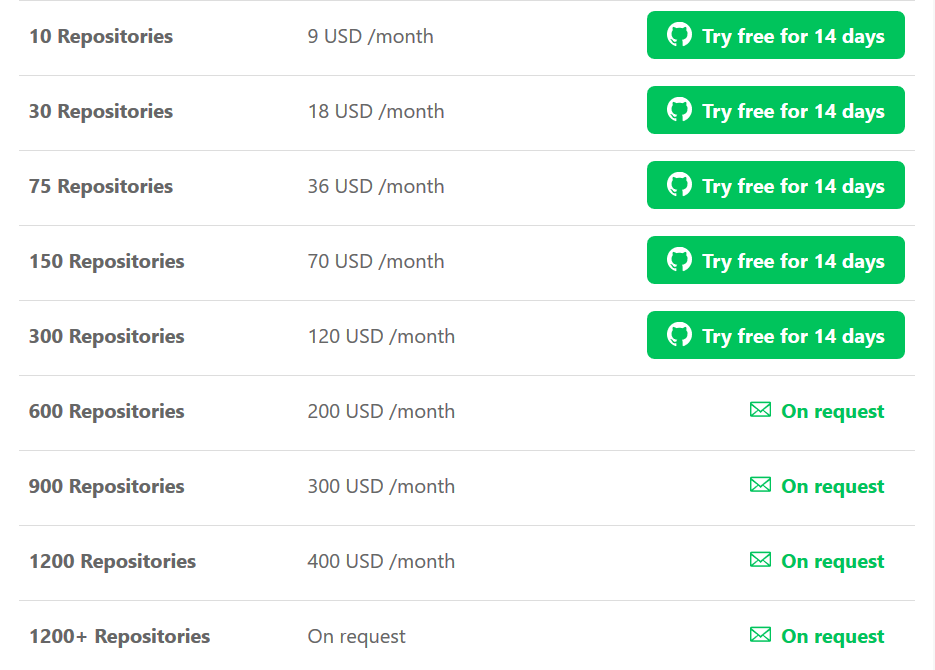
\includegraphics[scale=0.38]{priceg.PNG}
			\end{center}
		\end{figure}

	\end{frame}                           



	\begin{frame} 				% frame 9
		\frametitle{Cijene usluga (Bitbucketa)}

		\begin{itemize}
			\item s besplatnom verzijom dobijemo javne i privatne repozitorije s najviše 5 članova
			\item dostupne su nam 3 verzije Bitbucketa: 
			

		\end{itemize}

		\begin{figure}
			\begin{center}
				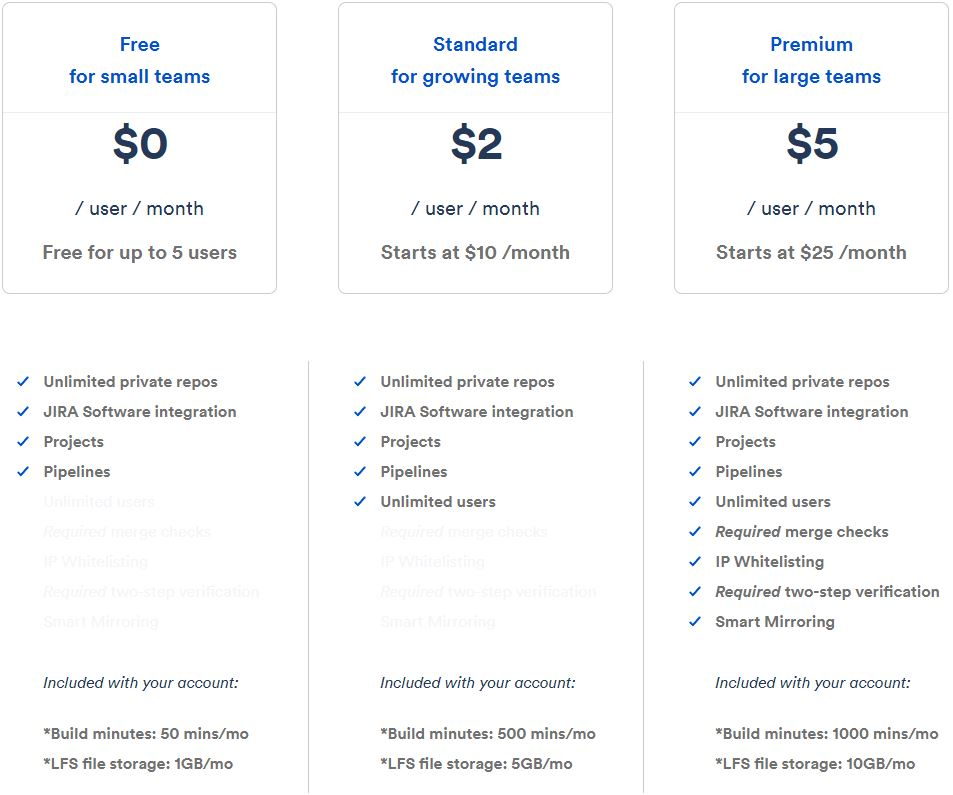
\includegraphics[width=8cm, height=5.5cm]{priceb.png}
			\end{center}
		\end{figure}
	\end{frame}




	\begin{frame}				% frame 10
		\frametitle{Usporedba}
		\begin{itemize}
			\item kod GitHub-a dobijemo beskonačni broj korisnika 
			\item ako koristimo besplatnu verziju dobijemo samo javne repozitorije, a ako hoćemo privatne onda moramo platiti
			\item cijena raste ovisno o broju repozitorija
			\item kod Bitbucket-a dobijemo uvijek beskonačno javnih i privatnih repozitorija
			\item plaća se po svakom korisniku, a cijena se snižava s vremenom

		\end{itemize}

	\end{frame}



	\begin{frame}				% frame 11
		\frametitle{Usporedba}

		\begin{itemize}
			\item ako imamo puno korisnika, a mali broj repozitorija onda se više isplati uzeti GitHub
			\item ako imamo puno repozitorija, a mali broj korisnika onda se više isplati uzeti Bitbucket
			\item ako imamo puno korisnika i repozitorija onda nam se vjerojatno više ispalti uzeti GitHub (ovisno o ugovoru)

		\end{itemize}


	\end{frame}

	\begin{frame}				% frame 12
		\frametitle{Verzije GitHub-a}
		\begin{itemize}
			\item GitHub Enterprise - za velike projekte
			\item GitHub - za prosječne veličine projekata
			\item Gists - za više manjih projekata

		\end{itemize}

	\end{frame}



	\begin{frame}				% frame 13
		\frametitle{Obrazovni program}
		\begin{itemize}
			\item GitHub Student Developer Pack
			\item kako bi se studentima omogućio besplatan pristup popularnim razvojnim alatima i uslugama
			\item firme koje su sudjelovale: Bitnami, Crowdflower, DigitalOcean, DNSimple, Unreal Engine,...

		\end{itemize}


	\end{frame}



	\begin{frame}				% frame 14
		\frametitle{Prednosti GitHub-a}
		\begin{itemize}
			\item 

		\end{itemize}


	\end{frame}




\end{document}

